\section{Requirements Engineering}
Ha come obiettivo la comprensione di come una soluzione software, che stiamo sviluppando, si deve comportare per risolvere un determinato problema. Bisogna quindi comprendere quale sia il problema da risolvere e in quale contesto si verifica, per poter arrivare così ad una soluzione corretta ed efficace di problemi reali.\\
Ci andiamo quindi a concentrare su due elementi essenziali: il problema e il contesto in cui il problema si verifica. \\

Stiamo usando una analogia per dire che all'interno del mondo possiamo avere un problema che risolviamo attraverso una macchina(computer)
\subsection{The problem world and the machine solution}
Definiamo le componenti della nostra analogia:
\begin{itemize}
    \item il \textbf{mondo}: presenta un problema derivante e prodotto dal mondo reale, che bisogna risolvere con un calcolatore. Il mondo è composto da:
        \begin{itemize}
            \item \textbf{componenti umani}, quindi staff, operatori, organizzazioni $\dots$
            \item \textbf{componenti fisici} che possiao pensare come device, software legacy, madre natura
        \end{itemize}
    \item \textbf{macchina}: bisogna svilupparla per risolvere il problema. Si compone di un software da sviluppare o comprare e implementazioni hardware associate con device di input e output annessi.
\end{itemize} 
RE si occupa proprio di definire gli effetti della macchina sul problema (sul mondo) identificato, e di definire le assunzioni che possiamo fare nel realizzare la macchina e quali sono le proprietà principali del mondo da prendere in considerazione.
RE studia quindi il mondo e la sua interazione con la macchina, senza definire come funziona internamente la macchina.\\
Ci sono alcuni componenti che costituiscono il \textbf{world phenomena} ed alcuni il \textbf{machine phenomena}, alcuni aspetti però sono condivisi tra le due componenti i \textbf{shared phenomena}.

Quando parliamo di RE è bene distinguere due elementi 
\begin{enumerate}
    \item ogni volta che si prende in considerazione un problema, normalmente esiste sempre un \textbf{system-as-is}, ovvero un sistema preesistente che già risolve il problema (anche se magari in modo non efficiente e qualitativamente insufficiente). Si ha quindi sempre un sistema da cui partire.
    \item il \textbf{system-to-be} è il sistema che si andrà a realizzare, in altre parole è il sistema su cui opererà la \textbf{macchina/software}.
\end{enumerate}
Studiare il \textbf{system-as-is} è essenziale per poter lavorare al \textbf{system-to-be}.

RE è un insieme di attività che hanno come obiettivo quello di esplorare, valutare, documentare, consolidare, rivisitare e adattare gli obiettivi, le capacità, le qualità, i vincoli e le assunzione su un software \textup{system-to-be} basate sul problema sorto dal \textbf{system-as-is } e sulle nuove opportunità tecnologiche.
L’output di queste attività è un \textbf{documento di specifica dei requisiti} con tutto ciò che il sistema deve soddisfare. Se l’output non è un singolo documento si ha una collezione di singoli requisiti, che nel metodo agile sono storie/cards e in altri metodi un repository centrale con un db condiviso contenete i vari requisiti. \\

Altre persone hanno cercato di definire differentemente i requisiti, esplicitando che quando si tende a sviluppare un software se i requirements non sono ben definiti, ci possiamo ritrovare differente da quello desiderato. Risulta necessario capire bene il why, what e how:
\begin{enumerate}
  \item \textbf{why}, perché serve un nuovo sistema in base alle nuove condizioni
  \item \textbf{what}, quale feature del sistema soddisferà il contesto in cui ci troviamo
  \item \textbf{who}, come il sistema deve essere costruito 
\end{enumerate}
RE si occupa degli obiettivi del \textbf{mondo}, per funzioni di vincoli sui sistemi software; e i loro collegamento a specifiche precise del come il software dovrebbe comportarsi. 

In un modello simil-cascata di sviluppo software, l'attività di RE è una delle primissime attività svolte (probabilmente la prima dal punto di vista tecnico), subito dopo quelle di definizione del sistema e di business plan. 
Re si occupa di capire qual è il giusto sistema da sviluppare, prima ancora di pensare al design, all’implementazione e all’evoluzione software, che invece si occupano di ottenere il software giusto, sviluppandolo nel modo corretto.

Sbagliare nell’attività di RE può portare ad un ottimo software che risolve i problemi sbagliati (o non tutti i problemi che dovrebbe risolvere). Lavorare sulla parte di RE è quindi molto difficile:
\begin{itemize}
    \item Si deve ragionare su tante versioni del sistema (broad scope): as-is, to-be e to-be-next (quando si vuole essere lungimiranti sul comportamento del sistema, sapendo e prevedendo evoluzioni future).
    \item Si lavora in ambienti ibridi (broad scope): tra umani, leggi, device, policy, leggi fisiche, quindi in un contesto eterogeneo che va compreso a fondo (ignorare degli aspetti può portare al fallimento).
    \item Si hanno diversi aspetti funzionali, qualitativi e di sviluppo (multiple concerns)
    \item Si hanno diversi livelli di astrazione (multiple abstraction levels): con obiettivi strategici a lungo termine di inserimento sul mercato e dettagli operazionali.
    \item Si hanno tanti stakeholders (multiple stakeholders): quindi diverse parti interessate per le quali risolvere problemi e considerare gli interessi (gestendo i potenziali conflitti tra i vari stakeholders).
    \item Si hanno tante attività tecniche legate tra loro (multiple interwined tasks): conflict management, risk management, evaluation of alternatives, prioritization, quality assurance, change anticipation (per capire cosa fare, in che ordine, con che rischi, con che livelli di qualità).
\end{itemize}


\subsection{Lo scope di RE: la dimensione del why, what e who}
\begin{enumerate}
    \item \textbf{dimensione del why}(why a new system?): dove si identificano, analizzano e rifiniscono i requisiti del \textbf{system-to-be} per: affrontare le carenze analizzate del \textbf{system-as-is}, in linea con gli obiettivi di business, sfruttando le opportunità tecnologiche.\\ 
    Si hanno le seguenti difficoltà:
      \begin{itemize}
        \item acquisire conoscenza del dominio 
        \item valutare opzioni alternative (ad esempio modi alternativi per soddisfare lo stesso obiettivo) 
        \item abbinare problemi-opportunità e valutarli in termini di implicazioni, e rischi associati 
        \item gestire obiettivi contrastanti
      \end{itemize}
    \item \textbf{dimensione del what}(what service?), dove si identificano, analizzano e rifiniscono le funzionalità del \textbf{system-to-be} (servizi software e associate procedure manuali) per soddisfare gli obiettivi individuati in base a vincoli di qualità: sicurezza, prestazioni, $\dots$ basati su ipotesi realistiche sull'ambiente.\\
    Si hanno le seguenti difficoltà:
        \begin{itemize}
            \item identificare il giusto set di funzionalità 
            \item specificarle precisamente per essere comprese da tutte le parti 
            \item garantire la tracciabilità $backward$ per gli obiettivi del sistema. (tornare indietro)
        \end{itemize}
    \item \textbf{dimensione del who}(who will be responsible for what?), dove si assegna responsabilità per gli obiettivi, i servizi, i vincoli tra i componenti del \textbf{system-to-be} in base alle loro capacità e agli obiettivi del sistema, uscendo anche dai confini dell'ambiente software.\\
    La difficoltà è valutare opzioni alternative per decidere il giusto grado di automazione 
\end{enumerate}

\subsection{Tipi di requisiti}
Bisogna anche ragionare sui tipi di requisiti su cui si deve lavorare. Una prima differenza si ha nel modo in cui sono scritti i requisiti:
\begin{itemize} 
    \item \textbf{descriptive statements (\textit{dichiarazioni descrittive})}, che indicano dei requisiti non negoziabili, rappresentano dei comportamenti derivanti dalle leggi del mondo su cui lavora la macchina. Si ha quindi zero margine di modifica 
    \item \textbf{prescriptive statements (\textit{dichiarazioni prescrittive})}, che indicano requisiti negoziabili che riguardano comportamenti che un sistema deve avere ma che volendo possono essere modificati. 
\end{itemize}
Si possono avere requisiti non ovvi, o lo sono solo in un contesto specialistico e quindi spesso non a chi lavora sul software (che generalmente non è del settore).

I requisiti possono inoltre differire per gli elementi che prendono in considerazione:
\begin{itemize}
  \item \textbf{system requirements},  riguardano il comportamento dell’ambiente, per capirne il funzionamento (che andrà ad influenzare il software).
  \item \textbf{software requirements}  riguardano il comportamento del software nell’ambiente, studiando i cosiddetti shared phenomena accennati in precedenza.
\end{itemize}
I requisiti non riguardano mai il comportamento interno del software. Ricordando che: 
\begin{itemize}
    \item $sistema = ambiente + software$
    \item $requisiti \; del \; sistema = requisiti \; software + domain \; properties + assunzioni$
\end{itemize}\label{riferimento}
Dove domain properties sono le leggi valide per un certo ambiente, proprietà immutabili e le assunzioni, che chi realizza il software, su come è fatto l’ambiente. Le assunzioni descrivono gli ambienti compatibili con il software. Se troppo restrittive possono portare al fallimento del progetto che riguarderebbe pochissimi casi particolari.\\

In ottica di un ragionamento di interazione tra sistema software e ambiente citiamo il \textbf{modello Parnas95}, della metà degli anni novanta. In modo elementare, il modello schematizza l’interazione software-ambiente in modo da esplicitare i device usati dal software-to-be per interagire con ambiente. 
\begin{figure}[H]
    \centering
    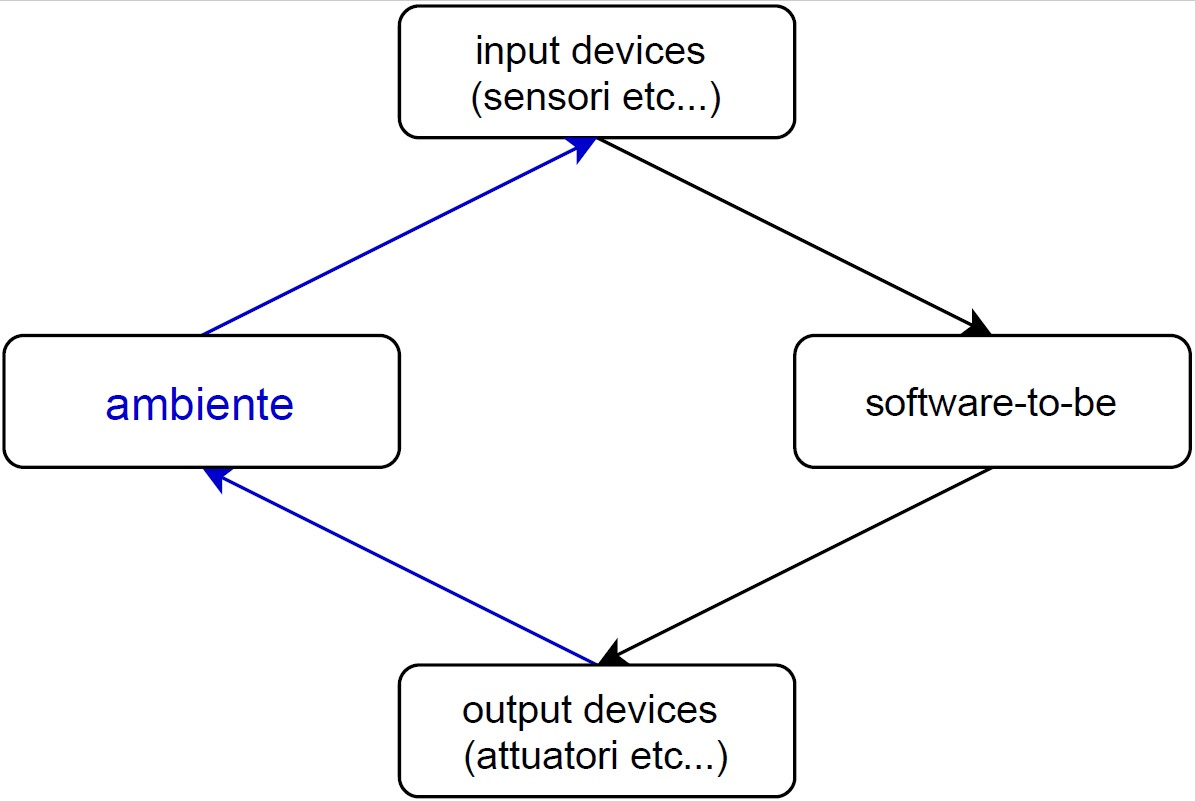
\includegraphics[scale= 0.25]{Imm/re_cose.PNG}
    \caption{Modello Parns95}
    \label{fig:parnas}
\end{figure}
Si ha uno schema composto da:
\begin{itemize}
    \item dei device di input, simil sensori, che percepiscono l’ambiente.
    \item dei device di output che permettono di interagire con l’ambiente.
\end{itemize}
e 4 tipi di variabili:
\begin{enumerate}
  \item \textbf{input data (I)}, tra \textit{input devices} e \textit{software-to-be}
  \item \textbf{output results (O)}, tra \textit{software-to-be} e \textit{output devices}
  \item \textbf{controlled variables  (C)}, tra \textit{output devices} e \textit{ambiente}
  \item \textbf{monitored variables (M)}, tra \textit{ambiente} e \textit{input devices}
\end{enumerate}
E si ha che $\mbox{System requirements}\subseteq M\times C$ e $\mbox{Software requirements}\subseteq I\times O$. Ritornando al comportamento di un software [\ref{riferimento}] avevamo parlato brevemente di dominio e assunzioni. Diremo inoltre che :\\
$\mbox{Assumptions}\subseteq M\times C\cup M\times I \cup C\times O$ \\
Definiamo \textbf{domain property} come un \textit{descriptive statement} sui problemi legati ai fenomeni del \textit{mondo} (a prescindere da qualsiasi \textbf{software-to-be}).\\ Utilizzando le 4 variabili diremo:
  $$\mbox{Domain property}\subseteq M\times C \mbox{, le leggi non possono essere infrante}$$

In conclusione si dirà che:
$$\mbox{Software requirements}= \textnormal{Map(System requirements,  Domain  property,  Assumptions)}$$

Abbiamo una distinzione delle categorie di requisiti, e le distinguiamo in due categorie principali:
\begin{enumerate}
    \item \textbf{Requisiti funzionali}: indicano le funzionalità che un sistema,\textbf{ system-to-be,} deve implementare, cosa deve essere in grado di fare. Non sono prevedibili prima di studiare il sistema.
    \item \textbf{Requisiti non funzionali}: indicano delle qualità o dei vincoli (in termini prestazioni, sicurezza, qualità) sulle funzionalità e quindi sui requisiti funzionali. Questa famiglia di aspetti non funzionali è più o meno standard.
\end{enumerate}

Si ha quindi una tassonomia per gli aspetti non funzionali tale per cui una volta individuate le funzionalità da implementare usiamo la tassonomia e chiederci se è  rilevante per il nostro progetto o per alcune delle funzionalità che vogliamo implementare. Se così fosse andiamo ad aggiungere dei requisiti non funzionali all'interno del nostro insieme di requisiti. 
Per alcuni tipi di progetti i requisiti funzionali e non sono difficilmente distinguibili, spesso mischiandosi.

\subsection{Qualità dei requisiti}
Le qualità sono obiettivi che i requisti devono  centrare:
\begin{itemize} 
    \item \textbf{completezza} di quanto descriviamo, descrivendo tutti i requisiti rilevanti del progetto, identificando tutti i comportamenti del sistema e documentarli in modo accurato. È una qualità virtualmente irraggiungibile in modo assoluto, non è infatti verificabile se il nostro insieme di requisiti sia completo.\\ Inoltre i requisiti variano al proseguire del progetto, interagendo anche con gli stakeholders, rendendo questo uno degli aspetti più difficili da studiare.
    \item \textbf{consistenza} dei requisti, senza conflitti. Nella mole di requisiti si possono purtroppo facilmente introdurre inconsistenze.
    \item \textbf{non ambiguità} di ciò che si scrive. Tutto deve essere chiaro e non soggetto ad interpretazione 
    \item \textbf{misurabilità}, quando rilevante, e quindi non basato su interpretazioni vaghe ma su misure concrete e specifiche 
    \item \textbf{fattibilità}, ovvero non si devono avere requisiti basati su funzionalità irrealizzabili 
    \item \textbf{comprensibilità} 
    \item \textbf{buona struttura}
    \item \textbf{modificabilità}, con possibilità di avere il risultato mantenibile del tempo 
    \item \textbf{tracciabilità} è importante tracciare tutti gli artefatti ottenibili come conseguenza di un certo requisito. Si tracciano anche le dipendenze tra requisiti.
\end{itemize}
Vediamo quindi gli errori che si fanno quando si va ad identificare i requisiti,per poter poi studiare tecniche per evitare, nel limite del possibile, tali errori possono essere:
\begin{itemize}
  \item \textbf{omissioni}, non riuscendo ad identificare qualche requisito. Anche un riconoscimento tardivo è un problema in quanto comporta la modifica del progetto, non sempre facile.
  \item \textbf{contraddizioni}, avendo conflitti tra i requisiti.
  \item \textbf{inadeguatezza}, avendo requisiti che non sono adeguati per un determinato problema.
  \item \textbf{ambiguità}, avendo requisiti interpretabili.
  \item \textbf{non misurabilità} di certi requisiti (specialmente non funzionali), che comportano difficoltà di gestione, precludendo confronti etc$\ldots$ 
\end{itemize}

Si hanno anche altri tipi di errore, potenzialmente meno gravi, ma altrettanto diffusi ai quali prestaste attenzione:
\begin{itemize}
  \item essere \textbf{troppo specifici} nella definizione dei requisiti includendo anche comportamenti interni al software che non dovrebbero essere descritti in questa fase. Bisogna dire quali funzionalità bisogna realizzare, non come
  \item descrivere requisiti \textbf{non implementabili} considerando vincoli temporali o di budget
  \item descrivere requisti \textbf{complessi da leggere}, ad esempio con un uso eccessivo di acronimi che rende complessa la lettura dei rischi
  \item avere \textbf{poca struttura} nella stesura dei requisiti, a livello visivo. Un documento tecnico deve essere facile da gestire e da usare 
  \item se si produce un documento bisogna evitare di fare riferimento a requisiti che non sono stati ancora descritti, ovvero evitando il \textbf{forward reference}
  \item evitare \textbf{rimorsi} di non aver definito nel momento giusto certi concetti che magari erano stati usati, senza definizione, precedentemente. Questi vanno definiti all'inizio del documento (nelle slide si dice tra parentesi)
  \item evitare la \textbf{poco modificabilità} del documento. È buona norma avere delle costanti simboliche, definite all'inizio, a cui fare riferimento nel documento, in modo che un'eventuale modifica si rifletta su tutto il documento
  \item evitare l'\textbf{opacità/logica di fondo/razionale/motivazioni} dei requisti, in modo che sia chiaro il perché esso è stato incluso, portando a mettere in discussione requisiti in realtà sensati a cui si arriverebbe comunque dopo ulteriore analisi, dopo aver perso ulteriore tempo
\end{itemize}

\subsection{Processo RE}
\begin{enumerate}
    \item \textbf{Domain understanding $\&$ Elicitation}:
        \begin{itemize}
            \item \textbf{Domain understanding}:  
            studio del dominio applicativo (spesso sconosciuto e complesso) dell’applicazione da realizzare, dell’organizzazione che richiede il prodotto e del funzionamento del system-as-is (punti di forza e di debolezza). Viene esguita l'identificazione degli stakeholders (e quindi tutte le parti interessate) del progetto per poter capire a fondo interessi e fini.\\
            In output si hanno le sezioni iniziali per la bozza di proposta preliminare e il glossario dei termini.
            \item \textbf{Requirements elicitation}: studio più approfondito del mondo, effettuando un’ulteriore analisi dei problemi legati al system-as-is, alla ricerca di sintomi, cause e conseguenze e identificando, grazie all’aiuto degli stakeholders: opportunità tecnologiche, condizioni del mercato, obiettivi di miglioramento, vincoli, organizzativi e tecnici, del system-as-is, alternative per raggiungere l’obiettivo e assegnare le responsabilità, scenari di ipotetica interazione software-ambiente, requisiti del software e assunzioni sull’ambiente.\\
            In questo caso l'output sono ulteriori sezioni per la bozza di proposta preliminare.
        \end{itemize}
    \item \textbf{Evaluation $\&$ agreement}\\Si effettuando decisioni basate sull’interazione con i vari stakeholders (che        spesso richiedono funzionalità conflittuali), occupandosi di:
        \begin{itemize}
            \item identificazione e risoluzione di conflitti di interesse
           \item identificazione e risoluzione di rischi legati al sistema proposto
           \item comparazione e scelta tra le alternative proposte in merito a obiettivi e rischi
           \item prioritizzazione dei requisiti, al fine di risolvere conflitti, definire vincoli di costi e tempi e supportare lo sviluppo incrementale.
        \end{itemize}
        Creando come output sezioni finali per la bozza di proposta preliminare, dove si documentano gli obiettivi selezionati, i requisiti, le assunzioni e il rationale, la logica di fondo delle opzioni selezionate.
    \item \textbf{Specification $\&$ documentation} \\In questa fase si raccoglie quanto fatto nelle prime due fasi per            produrre il documento, si punta ad avere quindi:
        \begin{itemize}
            \item una definizione precisa di tutte le funzionalità del sistema scelto, tra cui:
                \begin{itemize}
                    \item obiettivi, concetti, proprietà rilevanti del dominio d’interesse, requisiti del sistema, requisiti del software, assunzioni sull’ambiente e responsabilità
                    \item motivazioni e logica di fondo delle opzioni scelte
                    \item probabili evoluzioni del sistema ed eventuali variazioni
                \end{itemize}
            \item organizzazione di tutte le funzionalità in una struttura coerente
            \item documentazione del tutto in un formato comprensibile a tutte le parti, mettendo in allegato i costi, il piano di lavoro e i tempi di consegna del risultato.
        \end{itemize}
        Producendo come output un Requirements Document (RD).
    \item \textbf{Validation $\&$ verification}
        In questa fase si studia l’RD, ovvero la sua garanzia di qualità, analizzando varie attività:
        \begin{itemize}
            \item validazione: quanto contenuto nell’RD dev’essere adeguato con quanto si necessita.
            \item verifica: non ci devono essere omissioni o inconsistenze.
            \item correzione di eventuali errori e difetti.
        \end{itemize}
        In questo ultimo step si produce un RD consolidato.
\end{enumerate}
